\documentclass[handout,usenames,dvipsnames]{beamer} % To enable \pause: remove the "handout" preamble
\usetheme{Boadilla}
\usecolortheme{default}
\usepackage{pgfpages}
% \setbeameroption{hide notes} % Only slides
% \setbeameroption{show only notes} % Only notes
\setbeameroption{show notes on second screen=right} % Both
\setbeamertemplate{note page}{\pagecolor{yellow!5}\insertnote}\usepackage{palatino}

\usepackage[utf8]{inputenc}
\usepackage[round]{natbib}
\renewcommand*{\bibfont}{\scriptsize}
\usepackage{tikz}
\usepackage{wrapfig}

\DeclareMathOperator{\rank}{rank}
\DeclareMathOperator{\erank}{erank}
\DeclareMathOperator{\cl}{cl}
\DeclareMathOperator{\diag}{diag}
\DeclareMathOperator{\spn}{span}
% \newtheorem{theorem}{Theorem}
\newtheorem{assumption}{Assumption}
% \newtheorem{definition}{Definition}
\newtheorem{observation}{Observation}
% \newtheorem{corollary}{Corollary}
% \newtheorem{lemma}{Lemma}
\usepackage{dsfont}
\newcommand{\onefunc}{\mathds{1}}
\newcommand{\din}{{d_{\text{in}}}}
\newcommand{\dhid}{{d_{\text{hidden}}}}
\newcommand{\dout}{{d_{\text{out}}}}
\newcommand{\eps}{\epsilon}
\newcommand{\TODO}{\Red{TODO}}
\newcommand{\abs}[1]{\left|{#1}\right|}
\newcommand{\tr}[1]{\text{Tr}\left({#1}\right)}
\newcommand{\vect}[1]{\text{vec}\left({#1}\right)}
\newcommand{\opt}[1]{#1^\star}
\newcommand{\norm}[2][]{{\left\|{#2}\right\|_{#1}}}
%\newcommand{\norm}[1]{\left\|#1\right\|}
\newcommand{\snorm}[1]{\|#1\|} %small norm
\renewcommand{\angle}[2]{\measuredangle \left( #1, #2 \right)}
\newcommand{\bigangle}[2]{\measuredangle \left\big( #1, #2 \right\big)}
\newcommand{\Red}[1]{\colorbox{red}{#1}}
\newcommand{\set}[1]{\left\{{#1}\right\}}

\newcommand{\ba}{\mathbf{a}}
\newcommand{\be}{\mathbf{e}}
\newcommand{\bx}{\mathbf{x}}
\newcommand{\bw}{\mathbf{w}}
\newcommand{\bg}{\mathbf{g}}
\newcommand{\bb}{\mathbf{b}}
\newcommand{\bu}{\mathbf{u}}
\newcommand{\bv}{\mathbf{v}}
\newcommand{\bz}{\mathbf{z}}
\newcommand{\bc}{\mathbf{c}}
\newcommand{\br}{\mathbf{r}}
\newcommand{\bd}{\mathbf{d}}
\newcommand{\bp}{\mathbf{p}}
\newcommand{\bh}{\mathbf{h}}
\newcommand{\by}{\mathbf{y}}
\newcommand{\bn}{\mathbf{n}}
\newcommand{\bs}{\mathbf{s}}
\newcommand{\bq}{\mathbf{q}}
\newcommand{\bmu}{\boldsymbol{\mu}}
\newcommand{\balpha}{\boldsymbol{\alpha}}
\newcommand{\bbeta}{\boldsymbol{\beta}}
\newcommand{\btau}{\boldsymbol{\tau}}
\newcommand{\bxi}{\boldsymbol{\xi}}
\newcommand{\blambda}{\boldsymbol{\lambda}}
\newcommand{\bepsilon}{\boldsymbol{\epsilon}}
\newcommand{\bsigma}{\boldsymbol{\sigma}}
\newcommand{\btheta}{{\boldsymbol{\theta}}}
\newcommand{\bomega}{\boldsymbol{\omega}}
\newcommand{\Xcal}{\mathcal{X}}

\newcommand{\co}{{\cal O}}
\newcommand{\ca}{{\cal A}}
\newcommand{\cb}{{\cal B}}
\newcommand{\cd}{{\cal D}}
\newcommand{\cdb}{{\cal D}^{\rm b}}
\newcommand{\cc}{{\cal C}}
\newcommand{\ck}{{\cal K}}
\newcommand{\cq}{{\cal Q}}
\newcommand{\ce}{{\cal E}}
\newcommand{\ct}{{\cal T}}
\newcommand{\cg}{{\cal G}}
\newcommand{\ch}{{\cal H}}
\newcommand{\cm}{{\cal M}}
\newcommand{\ci}{{\cal I}}
\newcommand{\cj}{{\cal J}}
\newcommand{\cw}{{\cal W}}
%\newcommand{\cl}{{\cal L}}
\newcommand{\cf}{{\cal F}}
\newcommand{\cv}{{\cal V}}
\newcommand{\cp}{{\cal P}}
\newcommand{\cu}{{\cal U}}
\newcommand{\cx}{{\cal X}}
\newcommand{\cy}{{\cal Y}}
\newcommand{\cz}{{\cal Z}}
\newcommand{\cs}{{\cal S}}
\newcommand{\cn}{{\cal N}}
\newcommand{\calr}{{\cal R}}

\newcommand{\bbs}{{\mathbb S}}
\newcommand{\reals}{{\mathbb R}}
\newcommand{\nat}{{\mathbb N}}
\newcommand{\integers}{{\mathbb Z}}
\newcommand{\complex}{{\mathbb C}}
\newcommand{\zero}{{\mathbf{0}}}

% Style conventions
\newcommand{\true}[1]{{\textcolor{ForestGreen}{\textbf{#1}}}}




\title[Implicit Reg.: Rank Min. in ReLU Networks]{Implicit Regularization Towards Rank Minimization in ReLU Networks}
\author[Nadav Timor]{
    by Nadav Timor\newline
    Advisor: Prof. Ohad Shamir
}
\institute[Weizmann Institute]{Weizmann Institute of Science}
\date[January 2022]{January 2022}
% \logo{
\includegraphics[height=.75cm]{WeizmannLogo.png}}



\begin{document}



\frame{\titlepage}

\begin{frame}
    \frametitle{Implicit~Regularization Towards Rank~Minimization\\in ReLU~Networks}
    A joint paper under review @ ICML 2022,\\
    w/ Gal Vardi and Ohad Shamir.
\end{frame}



\section{What is implicit regularization?}

\begin{frame}{What is \emph{implicit regularization}?}{Generalization despite overparameterization}
    \pause
    \newline
    If \#[learnable parameters] $>>$ \#[training examples]:
    \pause
    \begin{itemize}
        \item \alert{Many} global minima w/ $0$ training loss.
        \pause
    \end{itemize}
    \pause
    \begin{block}{Phenomenon in practice (\cite{zhang2017understanding})}
        GD over such overparameterized neural networks generalize well even when trained \true{w/o~explicit~regularization}.
    \end{block}
    \textbf{Q:} How?\\
    \pause
    \textbf{Possible A:} \emph{``implicit regularization''} (or \emph{``implicit bias''}).
    
    \note{
        We focus on overparameterized neural networks, namely, 
        \begin{enumerate}
            \item there are far more learnable~parameters than training~examples.
            \item Then, we face an underdetermined optimization~problem with many global~minima of zero~training~loss.
            \item A central puzzle in the theory~of~deep~learning is how such overparameterized neural~networks generalize, even when trained without explicit regularization, as \cite{zhang2017understanding}  demonstrated.
            \item A possible explanation is that GD induces an {\em implicit~regularization}~(or~\emph{implicit~bias}).
        \end{enumerate}
        Today we take another step in trying to characterizing this regularization/bias.
        
        \vspace*{\fill}
        \noindent\rule{\textwidth}{1pt}
        \newline
        \alert{If asked:}
        \begin{itemize}
            \item \cite{zhang2017understanding}: Large CNNs,\\
            trained w/ stochastic~gradient~methods\\
            fit a random~labeling (of the training~data), or even completely~unstructured random~noise.\\
            Unaffected by explicit~regularization.
        \end{itemize}
    }
\end{frame}




\begin{frame}{What is \emph{implicit regularization/bias}?}
    \tikzset{every picture/.style={line width=0.75pt}} %set default line width to 0.75pt        
    
    \begin{tikzpicture}[x=0.75pt,y=0.75pt,yscale=-1,xscale=1]
        % uncomment if require: \path (0,261); %set diagram left start at 0, and has height of 261
        
        % 1. theta(0) := initial parameterization
        %Shape: Ellipse [id:dp021475373846624457] 
        \draw  [fill={rgb, 255:red, 148; green, 196; blue, 242 }  ,fill opacity=0.48 ] (6,128.75) .. controls (6,60.96) and (108.97,6) .. (236,6) .. controls (363.03,6) and (466,60.96) .. (466,128.75) .. controls (466,196.54) and (363.03,251.5) .. (236,251.5) .. controls (108.97,251.5) and (6,196.54) .. (6,128.75) -- cycle ;
        % Text Node
        \draw (109,24) node [anchor=north west][inner sep=0.75pt]  [font=\Large] [align=left] {$\displaystyle \mathbb{R}^{d}$};
        % Text Node
        \draw (338,28) node [anchor=north west][inner sep=0.75pt]  [font=\small] [align=left] {$\displaystyle \boldsymbol{\theta }(0)$};
        % Text Node
        \draw (377,46) node [anchor=north west][inner sep=0.75pt]  [font=\small] [align=left] {$\displaystyle \boldsymbol{\theta }(0)$};
        % Text Node
        \draw (405,64) node [anchor=north west][inner sep=0.75pt]  [font=\small] [align=left] {$\displaystyle \boldsymbol{\theta }(0)$};
        % Text Node
        \draw (426,89) node [anchor=north west][inner sep=0.75pt]  [font=\small] [align=left] {$\displaystyle \boldsymbol{\theta }(0)$};
        %Shape: Circle [id:dp6052897788269528] 
        \draw  [fill={rgb, 255:red, 0; green, 0; blue, 0 }  ,fill opacity=1 ] (343,44.5) .. controls (343,42.71) and (344.46,41.25) .. (346.25,41.25) .. controls (348.04,41.25) and (349.5,42.71) .. (349.5,44.5) .. controls (349.5,46.29) and (348.04,47.75) .. (346.25,47.75) .. controls (344.46,47.75) and (343,46.29) .. (343,44.5) -- cycle ;
        %Shape: Circle [id:dp38777159033159503] 
        \draw  [fill={rgb, 255:red, 0; green, 0; blue, 0 }  ,fill opacity=1 ] (383,62.5) .. controls (383,60.71) and (384.46,59.25) .. (386.25,59.25) .. controls (388.04,59.25) and (389.5,60.71) .. (389.5,62.5) .. controls (389.5,64.29) and (388.04,65.75) .. (386.25,65.75) .. controls (384.46,65.75) and (383,64.29) .. (383,62.5) -- cycle ;
        %Shape: Circle [id:dp2748850897412932] 
        \draw  [fill={rgb, 255:red, 0; green, 0; blue, 0 }  ,fill opacity=1 ] (411,80.5) .. controls (411,78.71) and (412.46,77.25) .. (414.25,77.25) .. controls (416.04,77.25) and (417.5,78.71) .. (417.5,80.5) .. controls (417.5,82.29) and (416.04,83.75) .. (414.25,83.75) .. controls (412.46,83.75) and (411,82.29) .. (411,80.5) -- cycle ;
        %Shape: Circle [id:dp7882824625742048] 
        \draw  [fill={rgb, 255:red, 0; green, 0; blue, 0 }  ,fill opacity=1 ] (432,105.5) .. controls (432,103.71) and (433.46,102.25) .. (435.25,102.25) .. controls (437.04,102.25) and (438.5,103.71) .. (438.5,105.5) .. controls (438.5,107.29) and (437.04,108.75) .. (435.25,108.75) .. controls (433.46,108.75) and (432,107.29) .. (432,105.5) -- cycle ;
        
        % 2. GF guarantee convergence to a local min.
        % 2.1. local- & global-min. 
        \pause
        %Shape: Ellipse [id:dp1447748006695847] 
        \draw  [fill={rgb, 255:red, 148; green, 180; blue, 242 }  ,fill opacity=0.5 ] (54,148) .. controls (54,100.23) and (140.86,61.5) .. (248,61.5) .. controls (355.14,61.5) and (442,100.23) .. (442,148) .. controls (442,195.77) and (355.14,234.5) .. (248,234.5) .. controls (140.86,234.5) and (54,195.77) .. (54,148) -- cycle ;
        %Shape: Ellipse [id:dp8297282672351468] 
        \draw  [fill={rgb, 255:red, 148; green, 160; blue, 242 }  ,fill opacity=0.61 ] (133,169) .. controls (133,138.9) and (191.87,114.5) .. (264.5,114.5) .. controls (337.13,114.5) and (396,138.9) .. (396,169) .. controls (396,199.1) and (337.13,223.5) .. (264.5,223.5) .. controls (191.87,223.5) and (133,199.1) .. (133,169) -- cycle ;
        % Text Node
        \draw (139,75) node [anchor=north west][inner sep=0.75pt]   [align=left] {local min.};
        % Text Node
        \draw (188,122) node [anchor=north west][inner sep=0.75pt]   [align=left] {0-loss (global min.)};
        
        % 2.2. GF & convergence
        %Shape: Circle [id:dp26530060350771567] 
        \draw  [fill={rgb, 255:red, 0; green, 0; blue, 0 }  ,fill opacity=1 ] (137.5,109.5) .. controls (137.5,107.71) and (138.96,106.25) .. (140.75,106.25) .. controls (142.54,106.25) and (144,107.71) .. (144,109.5) .. controls (144,111.29) and (142.54,112.75) .. (140.75,112.75) .. controls (138.96,112.75) and (137.5,111.29) .. (137.5,109.5) -- cycle ;
        %Shape: Circle [id:dp7555562235073366] 
        \draw  [fill={rgb, 255:red, 0; green, 0; blue, 0 }  ,fill opacity=1 ] (268,187.5) .. controls (268,185.71) and (269.46,184.25) .. (271.25,184.25) .. controls (273.04,184.25) and (274.5,185.71) .. (274.5,187.5) .. controls (274.5,189.29) and (273.04,190.75) .. (271.25,190.75) .. controls (269.46,190.75) and (268,189.29) .. (268,187.5) -- cycle ;
        %Shape: Circle [id:dp8780252532068147] 
        \draw  [fill={rgb, 255:red, 0; green, 0; blue, 0 }  ,fill opacity=1 ] (286,195.5) .. controls (286,193.71) and (287.46,192.25) .. (289.25,192.25) .. controls (291.04,192.25) and (292.5,193.71) .. (292.5,195.5) .. controls (292.5,197.29) and (291.04,198.75) .. (289.25,198.75) .. controls (287.46,198.75) and (286,197.29) .. (286,195.5) -- cycle ;
        %Shape: Circle [id:dp49477076878892456] 
        \draw  [fill={rgb, 255:red, 0; green, 0; blue, 0 }  ,fill opacity=1 ] (332,196.5) .. controls (332,194.71) and (333.46,193.25) .. (335.25,193.25) .. controls (337.04,193.25) and (338.5,194.71) .. (338.5,196.5) .. controls (338.5,198.29) and (337.04,199.75) .. (335.25,199.75) .. controls (333.46,199.75) and (332,198.29) .. (332,196.5) -- cycle ;
        % Shape: Circle
        \draw [shift={(144,109.5)}, rotate = 15] [fill={rgb, 255:red, 144; green, 19; blue, 254 }  ,fill opacity=1 ][line width=0.08]  [draw opacity=0] (8.93,-4.29) -- (0,0) -- (8.93,4.29) -- cycle    ;
        %Curve Lines [id:da13081269331006762] 
        \draw [color={rgb, 255:red, 144; green, 19; blue, 254 }  ,draw opacity=1 ]   (346.25,44.5) .. controls (193.77,-10.56) and (250.43,136.68) .. (145.59,109.92) ;
        %Curve Lines [id:da9648887968720957] 
        \draw [color={rgb, 255:red, 144; green, 19; blue, 254 }  ,draw opacity=1 ]   (386.25,65.75) .. controls (117,192.5) and (329,-49.5) .. (271,183.5) ;
        \draw [shift={(271,183.5)}, rotate = 283.98] [fill={rgb, 255:red, 144; green, 19; blue, 254 }  ,fill opacity=1 ][line width=0.08]  [draw opacity=0] (8.93,-4.29) -- (0,0) -- (8.93,4.29) -- cycle    ;
        %Curve Lines [id:da9531076976821162] 
        \draw [color={rgb, 255:red, 144; green, 19; blue, 254 }  ,draw opacity=1 ]   (414.25,80.5) .. controls (298.76,113.99) and (352.57,165.91) .. (295.2,194.22) ;
        \draw [shift={(292.5,195.5)}, rotate = 335.61] [fill={rgb, 255:red, 144; green, 19; blue, 254 }  ,fill opacity=1 ][line width=0.08]  [draw opacity=0] (8.93,-4.29) -- (0,0) -- (8.93,4.29) -- cycle    ;
        %Curve Lines [id:da952929077453363] 
        \draw [color={rgb, 255:red, 144; green, 19; blue, 254 }  ,draw opacity=1 ]   (435.25,108.75) .. controls (429.06,137.21) and (392.49,245.06) .. (339.61,200.89) ;
        \draw [shift={(338,199.5)}, rotate = 41.62] [fill={rgb, 255:red, 144; green, 19; blue, 254 }  ,fill opacity=1 ][line width=0.08]  [draw opacity=0] (8.93,-4.29) -- (0,0) -- (8.93,4.29) -- cycle    ;
        % Text Node
        \draw (243,22) node [anchor=north west][inner sep=0.75pt]  [color={rgb, 255:red, 144; green, 19; blue, 254 }  ,opacity=1 ] [align=left] {GF};
        % Text Node
        \draw (103,100) node [anchor=north west][inner sep=0.75pt]  [font=\small] [align=left] {$\displaystyle \boldsymbol{\theta }( \infty )$};
        % Text Node
        \draw (233,179) node [anchor=north west][inner sep=0.75pt]  [font=\small] [align=left] {$\displaystyle \boldsymbol{\theta }( \infty )$};
        % Text Node
        \draw (267.5,196.5) node [anchor=north west][inner sep=0.75pt]  [font=\small] [align=left] {$\displaystyle \boldsymbol{\theta }( \infty )$};
        % Text Node
        \draw (326.25,179.25) node [anchor=north west][inner sep=0.75pt]  [font=\small] [align=left] {$\displaystyle \boldsymbol{\theta }( \infty )$};
        
        % 3. When GF converges to a global min. (w.r.t. the loss): Can we guarantee to which one?
        \pause
        %Shape: Ellipse [id:dp2535016048578479] 
        \draw  [color={rgb, 255:red, 0; green, 0; blue, 0 }  ,draw opacity=1 ][fill={rgb, 255:red, 245; green, 166; blue, 35 }  ,fill opacity=0.6 ][dash pattern={on 5.63pt off 4.5pt}][line width=1.5]  (199,182.5) .. controls (199,164.83) and (236.83,150.5) .. (283.5,150.5) .. controls (330.17,150.5) and (368,164.83) .. (368,182.5) .. controls (368,200.17) and (330.17,214.5) .. (283.5,214.5) .. controls (236.83,214.5) and (199,200.17) .. (199,182.5) -- cycle ;
        % Text Node
        \draw (226,157) node [anchor=north west][inner sep=0.75pt]   [align=left] {implicit bias?};
    \end{tikzpicture}
    
    \note{
        Let's try to understand implicit regularization by the following illustration:
        \begin{enumerate}
            \item The points in $\reals^d$ that we marked by $\btheta(\zero)$ are different possible initial parameterizations of a neural network.
            \item We know that GF (e.g., w.r.t. square loss) guarantee convergence to a local minima. 
            \item The question is: When GF converges to a global minima, can we guarantee to which one?
        \end{enumerate}
        But please remember that the "implicit bias" we are looking for may not even exist!
    }
\end{frame}




\section{Square loss}
\subsection{Previous work}
\subsubsection{Linear networks}

\begin{frame}{Previous work}{Implicit regularization in linear networks}
    \pause
    \begin{definition}[fully-connected~neural~network]
        A fully-connected~neural~network $N_\btheta$ of depth~$k \geq 2$ is parameterized by a collection~$\btheta := [W^{(\ell)}]_{\ell=1}^k$ of weight~matrices\\
        ($\forall \ell \in [k] : W^{(\ell)} \in \reals^{d_\ell \times d_{\ell-1}}$), and computes a function $N_\btheta : \reals^\din \to \reals^\dout$:
        \[
            N_\btheta(\bx) := 
            \onslide<5->{W^{(k)}}
                \onslide<4->{\sigma\Big( W^{(k-1)} \ldots }
                    \onslide<3->{\sigma\Big( W^{(2)}~} 
                        \sigma\Big( W^{(1)} \bx \Big) 
                    \onslide<3->{\Big)}
                \onslide<4->{ \Big)} 
            \onslide<5->{\Big)}
            , \forall \bx
        \]
        where $\sigma:\reals \to \reals$ is an activation~function that acts coordinate-wise.
    \end{definition}
    \onslide<6->{
        \begin{description}
            \item[fully-connected \emph{linear} neural~network] $N_\btheta$, where $\sigma$ is the identity.
            \item[fully-connected \emph{ReLU} neural~network] $N_\btheta$, where $\sigma(z) := \max\set{0, z}$.
        \end{description}
    }
    \onslide<7->{
        \begin{block}{Matrix Factorization}
            What is the implicit regularization in training linear networks of depth 2 and multiple outputs w.r.t. square loss? ($W^{(2)}W^{(1)}\bx_i = W^* \bx_i, \forall i \in [n]$.)
        \end{block}
    }
    
    \note{
        \scriptsize
        In recent years, several works studied the relationship between the implicit~regularization in \emph{linear}~neural~networks and rank~minimization. To understand those, let's first define our model.
        \begin{enumerate}
            \itemsep=0pt
            \topsep=0pt
            \item We concern a fully-connected~neural~network, denoted by $N_\btheta$, where $\btheta$ is a collection of $k$ weight~matrices $W^{(\ell)}$. We say that $k$ is the \emph{depth} of the network, and it is $\ge 2$. The network computes a function $\reals^{\din} \to \reals^{d\out}$ in the following iterative way. A given input vector $\bx$ is multiplied by the first weight matrix, $W^{(1)}$. On the resulted multiplication, we apply an entrywise real-valued function, denoted by $\sigma$. This expression is called ``the output of the first layer" or ``the input to the second layer".
            \item Then, we repeat: We take the output of the first layer and do the same: Multiplying by $W^{(2)}$ and applying $\sigma$.
            \item This continues until we compute the input to the last layer.\\
            The $d_\ell$ rows of $W^{(\ell)}$ are ``the neurons of the $ell$-th layer". The \emph{hidden neurons} are the neurons in all layers except the last (namely, in layers $1, \ldots, k-1$). The \emph{width of the $\ell$-th layer} equals $d_\ell$ (the number of rows in $W^{(\ell)}$) and the \emph{width of the network} is the maximal width of its layers.
            \item Then, we only multiply by the last weight matrix, $W^{(K)}$. Note that we do not have an activation function in the last layer or bias terms.
            \item When referring to a \emph{linear} network, we mean that $\sigma$ is the identity function. \emph{ReLU} network is when $\sigma$ is the $\max$ between $0$ and its input.
            \item A main focus in recent years was on the matrix~fact.~problem, which corresponds to training a depth-2~linear~network with multiple outputs w.r.t. the square~loss. Think of finding $W^{(1)}, W^{(2)}$ that realize the training dataset, given by $\bx_i$ and $W^*$. The matrix~factorization~problem is considered a well-studied test-bed for analyzing implicit~regularization in DL.
        \end{enumerate}
    }
\end{frame}



\begin{frame}
    \begin{definition}[square loss]
        Given a network $N_\btheta$ and a dataset $\{(\bx_i,\by_i)\}_{i=1}^n \subseteq \reals^\din \times \reals^\dout$,
        \begin{align} \label{eq:objective}
        	 L_{X,Y}(\btheta) 
        	 := \frac{1}{2} \sum_{i=1}^n \norm{N_\btheta(\bx_i) - \by_i}^2
        	 = \frac{1}{2} \norm{N_\btheta(X) - Y}_F^2~.
        \end{align}
        $(X,Y) \in \reals^{\din \times n} \times \reals^{\dout \times n}$ are the corresponding data matrices.
    \end{definition}
    \pause
    \begin{itemize}
        \item Overparameterization $\Rightarrow$
        \pause
        \begin{itemize}
            \item $\min_\btheta L(\btheta)=0$.
            \item $L$ has multiple (or even infinitely many) global minima.
        \end{itemize}
    \end{itemize}
    \pause
    \begin{definition}[gradient flow (GF) w.r.t. square loss]
        Let~$\btheta(t)$ be the trajectory of GF. Starting from $\btheta(0)$, the dynamics is given by $\frac{d \btheta(t)}{dt} = -\nabla L_{X,Y}(\btheta(t))$.
    \end{definition}
    \begin{itemize}
        \item Behaves as GD w/ an infinitesimally small step~size.
        \pause
        \item GF \emph{converges} $\Leftrightarrow \lim_{t \to \infty}\btheta(t)$~exists. Then, $\btheta(\infty) := \lim_{t \to \infty}\btheta(t)$.
        \pause
        \item We assume $\sigma'(0) = 0$ for convenience.
    \end{itemize}
    
    \note{
        \begin{enumerate}
            \item \true{Empirical} square loss.
            \item Our assumption that $\sigma'(0) = 0$:\\
            Practical implementations of gradient~methods define $\sigma'(0) \in [0,1]$.
        \end{enumerate}
    }
\end{frame}



\begin{frame}{Implicit bias in linear~networks: Matrix~fact.}
    \pause
    \begin{block}{\cite{gunasekar2018implicit}’s conjecture \onslide<3->{\hfill\alert{X}}}
        The implicit~bias in \emph{matrix~fact.} can be characterized by the \alert{nuclear~norm} of the corresponding linear~predictor.
    \end{block}
    \pause
    \begin{itemize}
        \item \alert{Formally refuted} by \cite{li2020towards}.
    \end{itemize}
    \pause
    \begin{block}{\cite{razin2020implicit}’s conjecture}
        (1) \emph{Matrix~fact.} is implicitly biased towards \true{low-rank}. (2) Some notion of rank~min. may be key to explaining generalization in deep~learning.
    \end{block}
    \pause
    \begin{exampleblock}{\cite{li2020towards} \hfill\checkmark}
        \emph{Matrix~fact.} is implicitly biased towards low-rank.
    \end{exampleblock}
    \pause
    \begin{exampleblock}{\cite{razin2021implicit}’s theoretical \& empirical results \hfill\checkmark}
        \emph{Tensor~fact.} (a generalization) is implicitly biased towards low-rank.
    \end{exampleblock}
    
    \note{
    \begin{enumerate}
        \item \cite{gunasekar2018implicit}’s conjecture:\\
        Was further studied in a string of works\\
        (e.g., \cite{belabbas2020implicit,arora2019implicit,razin2020implicit}).
    \end{enumerate}
    }
\end{frame}




\subsubsection{Nonlinear networks}



\begin{frame}{Implicit bias in nonlinear networks w/ square loss}{Neural~network~compression}
    \pause
    \begin{exampleblock}{Empirical evidences}
        Replacing the weight~matrices by low-rank~approximations $\Rightarrow$ only a small drop in accuracy.
        \newline \newline
        (cf., \cite{denton2014exploiting,yu2017compressing,alvarez2017compression,arora2018stronger,tukan2020compressed})
    \end{exampleblock}
    \pause
    \begin{itemize}
        \item This suggests: In~practice, weight~matrices are not too far from being low-rank.
        \pause
        \item Today: Are they \textbf{provably} behave this way?
    \end{itemize}
    \pause
    \newline \newline
    Our proofs:
    \begin{itemize}
        \item \alert{NO!} \pause (not always)
        \item BUT, in some reasonable settings, \true{YES}: sufficient depth $\Rightarrow$ low-rank bias.
    \end{itemize}
\end{frame}


\begin{frame}{Implicit bias in nonlinear networks w/ square loss}{More prior results...}
    \pause
    \begin{block}{\cite{oymak2019overparameterized}}
         GD over certain nonlinear models is guaranteed to converge to a 0-loss~solution w/ a bounded $\ell_2$~norm, under some assumptions.
    \end{block}
    \pause
    \begin{block}{\cite{vardi2021implicit}}
         In ReLU networks of width 1, $\forall$ regularization~function~$\calr(\btheta)$, if  GF w/ the square~loss converges to a global~minimum that minimizes~$\calr \Rightarrow \calr$ is \alert{trivial}. %($\btheta :=$ model's parameters.)
    \end{block}
    \pause
    \begin{itemize}
        \item $\Rightarrow$ $\not\exists$ a non-trivial~$\calr(\btheta)$ which expresses the implicit~bias for all possible datasets and initializations.
        \pause
        \item Does GF is implicitly~biased towards low-ranks? (\emph{rank} is undefined for width $1$.)
        \pause
        \item $\not\Rightarrow$ GF doesn't act as a \emph{heuristic} for rank~minimization (i.e., minimizes the ranks for ``most'' datasets and initializations).
    \end{itemize}
    
    \note{
    At the beginning:
    \begin{itemize}
        \item "Sol-tanol-kotabi"
    \end{itemize}
    At the end:\\More works:
    \begin{enumerate}
        \item \cite{williams2019gradient,jin2020implicit}:\\
        Dynamics \& implicit~bias of GD\\
        in wide~depth-$2$~ReLU~networks w/ \alert{input~dimension~$1$}.
    \end{enumerate}
    }
\end{frame}




\subsection{Our results}

\begin{frame}{Our results}{GF does~not even approximately minimize ranks}
    \pause
    Setting: \true{ReLU}~networks of depth $2$ and width $2$ w/ multiple outputs,\\
    \pause
    trained w/ the square~loss.
    \pause
    \begin{exampleblock}{\cite{li2020towards,razin2020implicit} (matrix/tensor~fact.)}
        \alert{Linear} networks of this architecture are implicitly biased towards low-rank. (GF can be viewed as a "heuristic for rank~minimization".)
    \end{exampleblock}
    \pause
    \begin{exampleblock}{Thm. (informal) \hfill\checkmark}
          GF does~not converge to a low-rank~solution for size-$2$ datasets, under mild assumptions on the dataset and initialization.
    \end{exampleblock}
    \pause
    \begin{itemize}
        \item $\Rightarrow$ No rank~minimization for ``most'' size-$2$ datasets.
    \end{itemize}
    \pause
    \begin{exampleblock}{Thm. (informal) \hfill\checkmark}
          W.p. at least constant, the solutions that GF converges to are not even close to have low~rank.
    \end{exampleblock}
\end{frame}



\begin{frame}
    \pause
    \begin{itemize}
        \item Setting: $(X, Y) \in \mathbb{R}^{2 \times 2} \times \mathbb{R}^{2 \times 2}$ (a training dataset), and $W,V\in \reals^{2 \times 2}$ s.t. $N_{W,V}(X)=V\sigma(WX)$ is a 0-loss~solution.
        \pause
        \item \emph{"low-rank"} $:= \rank W \leq 1$. Why?
        \pause
        \begin{itemize}
            \item $\rank Y = 2 \Rightarrow \rank V = 2$.\\(Since $\rank Y =\rank N_{W,V}(X)  \leq \rank V$).
            \pause
            \item Trivially, $\rank W \leq 2$.
        \end{itemize}
        \pause
        \item $\exists$ such a low-rank~0-loss~solution?
        \pause 
        \true{YES!}
    \end{itemize}
        \begin{exampleblock}{Thm.}
          $\forall$ labeled dataset $(X, Y) \in \mathbb{R}^{2 \times 2} \times \mathbb{R}^{2 \times 2}$ of inputs $\bx_1, \bx_2 \in \mathbb{R}^2$ s.t. $\measuredangle(\bx_1, \bx_2) > 0$, $\exists$ a 0-loss~solution $N_{W,V}$ with $W,V \in \reals^{2 \times 2}$ s.t. $\rank(W)=1$.
    \end{exampleblock}
    \pause
    Proof idea:
    \pause
    \begin{itemize}
        \item Construct (the weight~vectors of) the neurons in the $1$st~layer to have opposite directions (hence $\rank W = 1$), s.t. each neuron is active for exactly one input.
        \pause
        \item An appropriate choice of the $2$nd layer’s weights achieves 0~loss.
    \end{itemize}
    \pause
    Does GF converges to such solutions?
    \note{
        2nd click:
        \begin{itemize}
            \item To understand rank~minimization in this simple setting, we consider the rank of $W$ in a zero-loss~solution. Why?
        \end{itemize}
        After the 3rd click:
        \begin{itemize}
            \item Otherwise, this setting is trivial.
        \end{itemize}
    }
\end{frame}




\begin{frame}
    Does GF converges to low-rank solutions? \true{NO!}
    \pause
    Assuming:
    \pause
    \begin{assumption}\label{assumption:ys_linearly_independent}
        The two target~vectors~$\by_1, \by_2$ are on the unit~sphere~$\mathbb{S}^1$ and are linearly~independent.
    \end{assumption}
    \pause
    \begin{assumption}\label{assumption:xs_bounded_angle}
        The two inputs~$\bx_1, \bx_2$ are on the unit~sphere~$\mathbb{S}^1$ and $\frac{\pi}{2} < \measuredangle(\bx_1, \bx_2) < \pi$.
    \end{assumption}
    \pause
    \begin{exampleblock}{Thm. \hfill\checkmark}\label{T2}
        Let $(X,Y) \in \mathbb{R}^{2 \times 2} \times \mathbb{R}^{2 \times 2}$ be a labeled dataset that satisfies Assumptions~\ref{assumption:ys_linearly_independent},~\ref{assumption:xs_bounded_angle}.
        Consider GF w.r.t. the square~loss~$L_{X,Y}(W,V)$. Suppose that $W,V \in \reals^{2 \times 2}$ are initialized s.t. 
        $\norm{\bw_i(0)} < \min \left\{ \frac{1}{2}, \frac{\sqrt{3}}{2} \cos{\frac{\measuredangle(\bx_1, \bx_2)}{2}} \right\}$ 
        and $\norm{\bv_i(0)} < \frac{1}{2}$ for all $i \in \{1,2\}$. If GF converges to a $0$-loss~solution~$N_{W(\infty),V(\infty)}$, then $\rank W(\infty) = 2$.
    \end{exampleblock}
    \pause
    Does GF converge to a \alert{close-to-low-rank} solution?
    
    \note{
        A1:
        \begin{enumerate}
            \item The assumptions that $\bx_i,\by_i$ are of unit norm are mostly for technical convenience, and we believe that they are not essential.
        \end{enumerate}
        Thm.:
        \begin{enumerate}
            \item GF does~not minimize the rank even in a very simple setting where the dataset contains two inputs w/ angle larger than $\pi/2$\\
            (as long as the initialization point is sufficiently close~to~$0$). In particular, if the dataset is drawn from the uniform distribution on the sphere, then this condition holds w.p. $1/2$.
            \item At the end: While \thmref{T2} shows that GF does~not minimize the rank, it does~not rule~out the possibility that it converges to a solution which is close to a low-rank~solution.
            \begin{itemize}
                \item There are many ways to define such closeness, such as:
                \begin{itemize}
                    \item the ratio of the Frobenius and spectral~norms,
                    \item the Frobenius~distance from a low-rank~solution, or
                    \item the exponential of the entropy of the singular~values
                \end{itemize}
                \item However, for $2\times 2$~matrices they all boil down to either having the two rows of the matrix being nearly aligned or having at~least one of them very small (at~least compared to the other).
            \end{itemize}
        \end{enumerate}
    }
\end{frame}




\begin{frame}
    \begin{exampleblock}{Thm. \hfill\checkmark} \label{T3}
        Let $(X,Y) \in \mathbb{R}^{2 \times 2} \times \mathbb{R}^{2 \times 2}$ be a labeled dataset that satisfies Assumptions~\ref{assumption:ys_linearly_independent} and~\ref{assumption:xs_bounded_angle}.
        Consider GF w.r.t. the square loss~function $L_{X,Y}(W,V)$. Suppose that $W,V \in \reals^{2 \times 2}$ are initialized s.t. for all $i \in \{1,2\}$ we have $\bv_i(0) = \zero$, and $\bw_i(0)$ is drawn from a spherically~symmetric distribution with 
        \begin{align*}
            \norm{\bw_i(0)} 
            \leq \frac{\sqrt{3}}{2} \min \left\{ 
            \sin\left(\frac{\pi - \measuredangle(\bx_1,\bx_2)}{4} \right), 
            \sin \left(\measuredangle(\bx_1,\bx_2) - \frac{\pi}{2}\right)
            \right\} ~.
        \end{align*}
        Let $E$ be the event that GF converges to a 0-loss~solution~$N_{W(\infty),V(\infty)}$ s.t.
        \begin{itemize}
            \item[(i)] $\measuredangle \left( \bw_1(\infty), \bw_2(\infty) \right) \in \left[ \frac{\pi}{2} - \left(\measuredangle(\bx_1, \bx_2) - \frac{\pi}{2} \right), \frac{3\pi}{4} + \frac{\measuredangle(\bx_1, \bx_2) - \pi/2}{2} \right]$,
            \item[(ii)] $\norm{\bw_i(\infty)} \in \left( \frac{\sqrt{3}}{2}, \sqrt{ \frac{1}{4} + \frac{4}{3 \left(\sin \measuredangle(\bx_1, \bx_2) \right)^2 } } \right)$ for all $i \in \set{1, 2}$.
        \end{itemize}
        Then, $\Pr \left[E \right] \ge 2 \cdot \left(\frac{\measuredangle(\bx_1,\bx_2)}{2\pi} \right)^2$.
    \end{exampleblock}
    
    \note{
        Before: \\
        In the following theorem, we show that under the aforementioned assumptions, for any fixed dataset, with at~least constant probability, GF converges to a zero-loss~solution, where the two row vectors $w_i$ are bounded away from~$0$, the ratio of their norms are bounded, and the angle between them is bounded (away from~$0$ and from~$\pi$; all by explicit constants that depend just on the dataset and are large in general). Thus, with at least constant probability, GF does~not minimize any reasonable approximate notion of rank.
        \newline
        \newline
        After:\\
        We note that in \thmref{T3} the weights in the second layer are initialized to zero ($v_i(0) = \zero$), while in \thmref{T2} the assumption on the initialization is weaker. This difference is for technical convenience, and we believe that \thmref{T3} should hold also under weaker assumptions on the initialization, as the next empirical result demonstrates.
    }
\end{frame}




\begin{frame}{GF does~not even approximately minimize~ranks}{An empirical result}
    \begin{figure}[t]
        \begin{columns}
            \column{0.5\textwidth}
            \frame{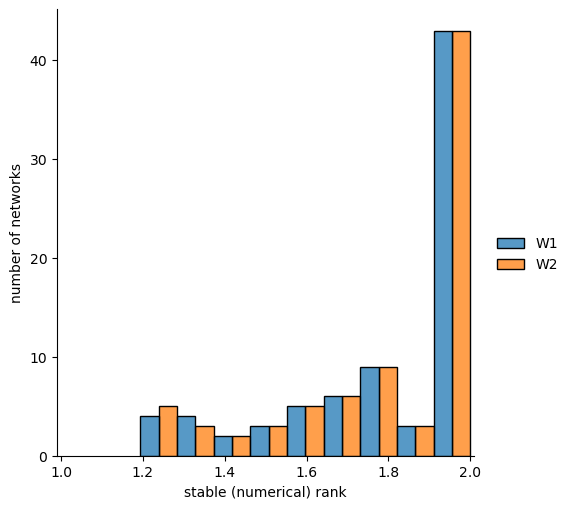
\includegraphics[scale=.45]{figures/final_f2s_displot.png}}
            
            \column{0.3\textwidth}
            \emph{"stable rank"} $:= {\norm{W^{(\ell)}}^2_F} / {\norm{W^{(\ell)}}^2_\sigma}$.
        \end{columns}
        \centering
        \caption{A histogram of the stable (numerical) ranks at convergence. In all runs, we converge to networks with stable~ranks which seem bounded away from $1$. Namely, GD does~not even approximately minimize the ranks.}
    \label{fig:empirical-high-f2s}
    \end{figure}
    
    \note{
        Start: Our theorems imply that for reasonable initialization schemes, GF will not converge close~to low-rank~solutions, with some positive~probability. We now present a simple experiment that corroborates this and suggests that, furthermore, this holds with~high~probability and for standard initializations.
        \newline \newline
        Only if asked: We trained ReLU~networks in the same setup as in the previous section (w.r.t. two $2\times 2$~weight~matrices~$W^{(1)},W^{(2)}$) on the two data~points~$\{(\bx_i,\by_i)\}_{i=1}^{2}$ where~$\by_1,\by_2$ are the standard~basis vectors in~$\reals^2$, and~$\bx_1,\bx_2$ are~$(1,0.99)$ and~$(-1,0.99)$ normalized to have unit~norm. At initialization, every row of~$W^{(1)}$ and every column of~$W^{(2)}$ is sampled uniformly~at~random from the sphere of radius~$10^{-4}$ around the origin. To simulate GF, we performed~$3\cdot 10^{6}$ epochs of full-batch~GD of step~size~$10^{-4}$, w.r.t. the square~loss. Of~$288$~repeats of this experiment, $79$~converged to negligible~loss~(defined~as~$<10^{-4}$). In 
        the figure, we plot a histogram of the \emph{stable~(numerical)~ranks} of the resulting weight~matrices, i.e. the ratio~${\norm{W^{(\ell)}}^2_F} / {\norm{W^{(\ell)}}^2_\sigma}$ of layer~$\ell \in [2]$. The figure clearly suggests that whenever convergence to zero~loss occurs, the solutions are all of rank~$2$, and none are even close~to being low-rank (in~terms of the stable~rank).
    }
\end{frame}



\begin{frame}{Proof ideas}
    Recall:
    \pause
    \begin{exampleblock}{Thm. \hfill\checkmark}\label{T2}
        Let $(X,Y) \in \mathbb{R}^{2 \times 2} \times \mathbb{R}^{2 \times 2}$ be a labeled dataset that satisfies Assumptions~\ref{assumption:ys_linearly_independent},~\ref{assumption:xs_bounded_angle}.
        Consider GF w.r.t. the square~loss~$L_{X,Y}(W,V)$. Suppose that $W,V \in \reals^{2 \times 2}$ are initialized s.t. 
        $\norm{\bw_i(0)} < \min \left\{ \frac{1}{2}, \frac{\sqrt{3}}{2} \cos{\frac{\measuredangle(\bx_1, \bx_2)}{2}} \right\}$ 
        and $\norm{\bv_i(0)} < \frac{1}{2}$ for all $i \in \{1,2\}$. If GF converges to a $0$-loss~solution~$N_{W(\infty),V(\infty)}$, then $\rank W(\infty) = 2$.
    \end{exampleblock}
    \begin{assumption}
        The two target~vectors~$\by_1, \by_2$ are on the unit~sphere~$\mathbb{S}^1$ and are linearly~independent.
    \end{assumption}
    \begin{assumption}
        The two inputs~$\bx_1, \bx_2$ are on the unit~sphere~$\mathbb{S}^1$ and $\frac{\pi}{2} < \measuredangle(\bx_1, \bx_2) < \pi$.
    \end{assumption}
\end{frame}



\begin{frame}
    \begin{columns}
            \column{0.5\textwidth}
            \begin{figure}[t]
                \centering
                \frame{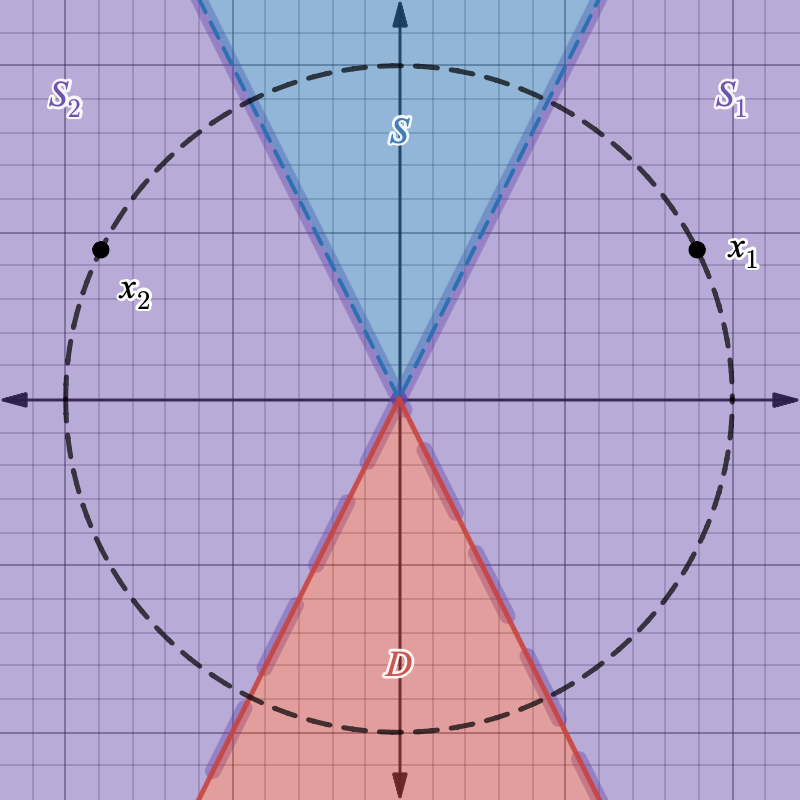
\includegraphics[scale=.25]{figures/D_and_Ss_regions.png}}
                \label{fig:D_and_Ss_regions}
            \end{figure}
            \pause
            \column{0.7\textwidth}
            {\fontsize{10}{10} \selectfont
            \begin{align*}
                &\mathcal{D} := \{ \bw \mid \forall i \in [2], \sigma(\bw^\top \bx_i) \le 0\}\\
                \pause
                &\mathcal{S} := \{ \bw \mid \forall i \in [2], \sigma(\bw^\top \bx_i) > 0 \}\\
                \pause
                &\mathcal{S}_j := \{ \bw  \mid  i=j \Leftrightarrow \sigma(\bw^\top \bx_i) > 0 \}
            \end{align*}
            }
    \end{columns}
    \pause
    {\fontsize{10}{10} \selectfont
    \[
        \mathcal{S}_1 := \{ \bw  \mid \sigma(\bw^\top \bx_1) > 0, \sigma(\bw^\top \bx_2) \leq 0\},
        \mathcal{S}_2 := \{ \bw  \mid \sigma(\bw^\top \bx_2) > 0, \sigma(\bw^\top \bx_1) \leq 0\}
    \]
    }
    
    \note{
        Intuitively,~$\mathcal{D}$~defines the ``dead''~region where neurons output~$0$ on both~$\bx_1,\bx_2$; $\mathcal{S}$~is the ``active''~region where a neuron outputs a positive~output on both~$\bx_1,\bx_2$; and $\mathcal{S}_1,\mathcal{S}_2$~are the ``partially~active''~regions, where the relevant neuron outputs a positive~output on one point, and~$0$ on the other. 
    }
\end{frame}



\begin{frame}
    \begin{columns}
        \column{0.6\textwidth}
        \begin{itemize}
            \setlength{\parskip}{0pt}
            \setlength{\abovedisplayskip}{0pt}
            \setlength{\belowdisplayskip}{0pt}
            \setlength{\abovedisplayshortskip}{0pt}
            \setlength{\belowdisplayshortskip}{0pt}
            
            \item Assume towards~contradiction:\\GF converges to some 0-loss~network~$N_{W(\infty),V(\infty)}$ s.t. ~$\rank(W(\infty))<2$. 
            \pause
            \item 0-loss $\Rightarrow Y = V(\infty) \sigma \left( W(\infty) X \right)$.
            \pause
            \item $\Rightarrow$ 
            \begin{align*}
                2 &= \rank(Y) = \rank \left( V(\infty) \sigma \left(W(\infty) X \right) \right) \\
                &\leq \rank \left( \sigma \left( W(\infty) X \right) \right).
            \end{align*}
        \end{itemize}    

        \column{0.4\textwidth}
        \begin{center}
            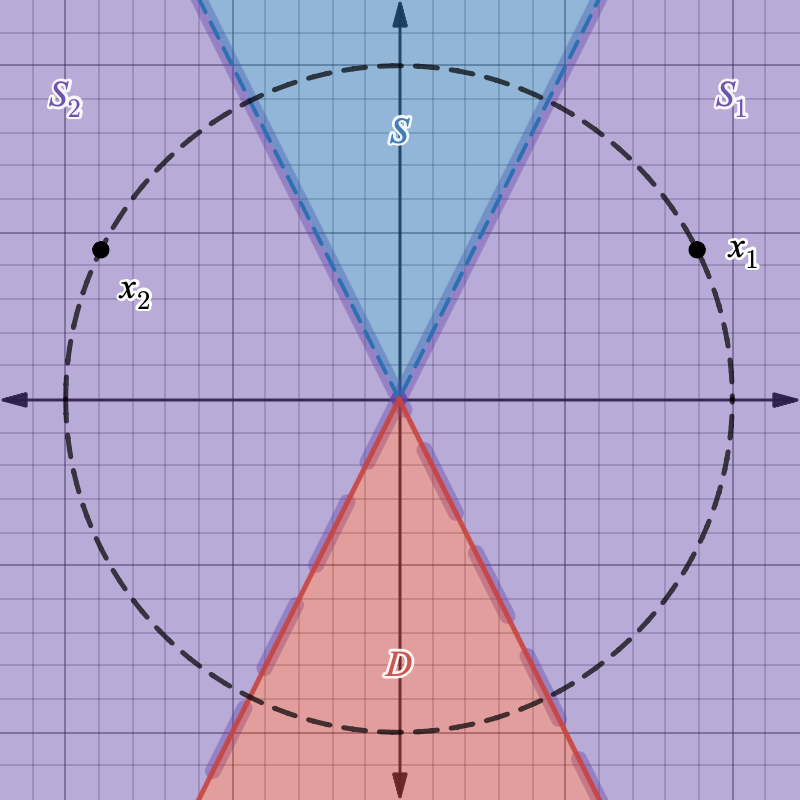
\includegraphics[width=\textwidth]{figures/D_and_Ss_regions.png}
        \end{center}
    \end{columns}
    
    \begin{itemize}
        \pause
        \item $\Rightarrow \bw_1(\infty), \bw_2(\infty) \notin \cd$. (Otherwise, $\zero^T$ is a row in~$\sigma(W(\infty) X)$.)
        \pause
        \item $\Rightarrow \bw_1(\infty), \bw_2(\infty) \ne \zero$ $\Rightarrow \rank(W(\infty))=1$. 
        \pause
        \item Denote $\bw_2(\infty) = \alpha \bw_1(\infty)$ where~$\alpha \neq 0$.
        \pause
        \begin{itemize}
            \item $\alpha > 0 \Rightarrow \sigma(\bw_2(\infty)^\top \bx_j) = \alpha \sigma(\bw_1(\infty)^\top \bx_j), \forall j \in [2] \Rightarrow$ contradiction!
            \pause
            \item $\Rightarrow \alpha < 0$.
        \end{itemize}
        \pause
        \item $\Rightarrow$ w.l.o.g., $\bw_1(\infty) \in \cs_1 \setminus \partial \cs_1, \bw_2(\infty) \in \cs_2 \setminus \partial \cs_2$.
    \end{itemize}
    
    \note{
        Starting from the 4th point: \newline
        \begin{itemize}
            \item Therefore, the weight~vectors~$\bw_1(\infty)$ and~$\bw_2(\infty)$ are~not in the region~$\cd$. Indeed, if $\bw_1(\infty)$ or~$\bw_2(\infty)$ are in~$\cd$, then at~least one of the rows of~$\sigma(W(\infty) X)$ is~zero, in~contradiction.
            \item In~particular, it implies that~$\bw_1(\infty)$ and~$\bw_2(\infty)$ are non-zero.
            \item Since by our assumption we have~$\rank(W(\infty))<2$, then we conclude that~$\rank(W(\infty))=1$. 
            \item We denote~$\bw_2(\infty) = \alpha \bw_1(\infty)$ where~$\alpha \neq 0$.
            \item Note that if~$\alpha > 0$, then~$\sigma(\bw_2(\infty)^\top \bx_j) = \alpha \sigma(\bw_1(\infty)^\top \bx_j)$ for~all~$j \in \{1,2\}$, in~contradiction
            \item Thus,~$\alpha < 0$.
            \item Since we also have~$\bw_1(\infty),\bw_2(\infty) \not \in \cd$, then one of these weight~vectors is in~$\cs_1 \setminus \partial \cs_1$ and the other is in~$\cs_2 \setminus \partial \cs_2$ (as can be seen in the figure). Assume~w.l.o.g. that~$\bw_1(\infty) \in \cs_1 \setminus \partial \cs_1$ and $\bw_2(\infty) \in \cs_2 \setminus \partial \cs_2$.
        \end{itemize}
    }
\end{frame}




\begin{frame}
    \begin{figure}[t]
        \centering
        \frame{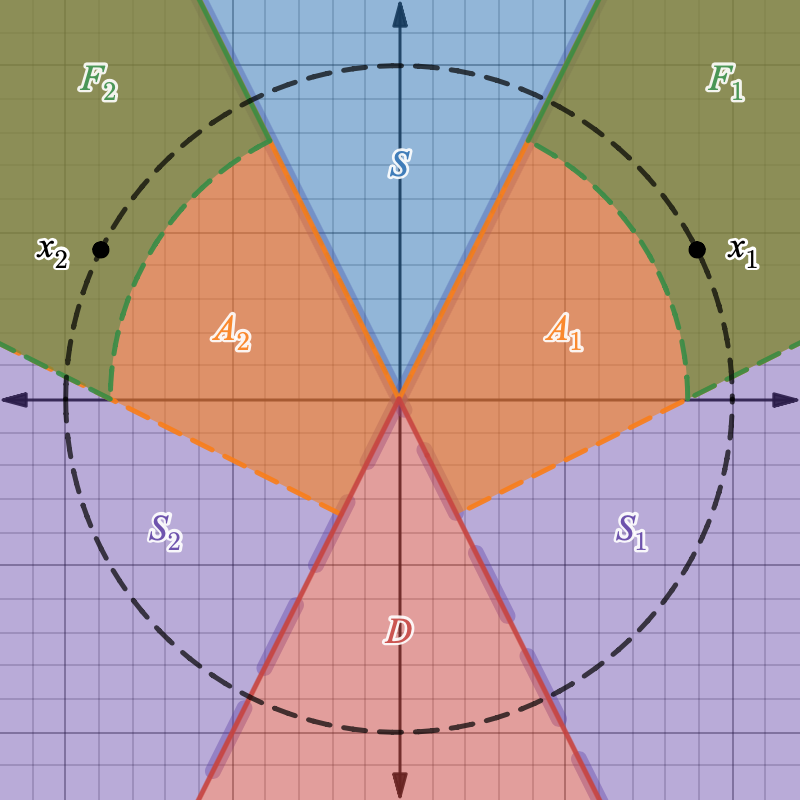
\includegraphics[scale=.25]{figures/F_and_A_regions.png}}
        \caption{Regions~$\cf_i$~(in~green) and~$\ca_i$ (the union of the green and orange regions). A dashed line marks an open~boundary.}
        \label{fig:F_and_A_regions}
    \end{figure} 

    \note{
        By observing the gradients of~$L_{X,Y}$ w.r.t.~$\bw_i$ for~$i \in \{1,2\}$, the following facts follow. First, if~$\bw_i(t) \in \cd$ at some time~$t$, then~$\frac{d}{dt} \bw_i(t) = \zero$, hence $\bw_i$~remains at~$\cd$ indefinitely, in~contradiction to~$\bw_i(\infty) \in \cs_i \setminus \partial \cs_i$. Thus, the trajectory~$\bw_i(t)$ does~not visit~$\cd$. Second, if~$\bw_i(t) \in \cs_i$ at time~$t$, then~$\frac{d}{dt} \bw_i(t) \in \spn\{\bx_i\}$. Since~$\bw_i(\infty) \in \cs_i \setminus \partial \cs_i$, we can consider the last~time~$t'$ that~$\bw_i$ enters~$\cs_i$, which can be either at the initialization (i.e.,~$t'=0$) or when moving from~$\cs$ (i.e.,~$t'>0$). For~all time~$t \geq t'$ we have~$\frac{d}{dt} \bw_i(t) \in \spn\{\bx_i\}$. It allows us to conclude that~$\bw_i(\infty)$ must be in a region~$\ca_i$ which is illustrated in \figref{fig:F_and_A_regions} (by the union of the orange and green regions).
        
        Furthermore, we show that~$\norm{\bw_i(\infty)}$ cannot be too~small, namely, obtaining a lower~bound on~$\norm{\bw_i(\infty)}$. First, a theorem from \cite{du2018algorithmic} implies that~$\norm{\bw_i(t)}^2 - \norm{\bv_i(t)}^2$ remains constant throughout the training. Since at the initialization both~$\norm{\bw_i(0)}$ and~$\norm{\bv_i(0)}$ are small, the consequence is that~$\norm{\bv_i(\infty)}$ is small if~$\norm{\bw_i(\infty)}$ is small.
        Also, since~$N_{W(\infty),V(\infty)}$ attains zero~loss and~$\bw_i(\infty) \in \cs_i$ for all $i \in \{1,2\}$, then we have~$\by_i = \bv_i(\infty) (\bw_i(\infty)^\top \bx_i)$, namely, only the $i$-th~hidden~neuron contributes to the output of~$N_{W(\infty),V(\infty)}$ for the input~$\bx_i$. Since~$\norm{\by_i}=\norm{\bx_i}=1$, it is impossible that both~$\norm{\bw_i(\infty)}$ and~$\norm{\bv_i(\infty)}$ are small. Hence, we are able to obtain a lower~bound on~$\norm{\bw_i(\infty)}$, which implies that~$\bw_i(\infty)$ is in a region~$\cf_i$ which is illustrated in \figref{fig:F_and_A_regions}.
        
        Finally, we show that since $\bw_1(\infty) \in \cf_1$ and $\bw_2(\infty) \in \cf_2$ then the angle between $\bw_1(\infty)$ and $\bw_2(\infty)$ is smaller than $\pi$, in~contradiction to $\bw_2(\infty) = \alpha \bw_1(\infty)$.
    }
\end{frame}




\begin{frame}{Our results}{Rank~min. in deep~networks w/ small~$\ell_2$~norm}
    \pause
    Settings: ReLU~networks, overparameterized in \true{depth}, of width $\ge 2$, trained w/ the square~loss.
    \pause
    \begin{exampleblock}{Thm. (informal)}
        For sufficiently deep networks, if $\btheta(\infty)$ exists and $\btheta(\infty) \in \arg\min_{\btheta} \norm{\btheta}$ s.t. $L_{X,Y}(\btheta(\infty)) = 0$, then 
        \[
        \frac{1}{k}\sum_{i=1}^{k} \frac{\norm{W^{(i)}(\infty)}_\sigma}{\norm{W^{(i)}(\infty)}_F}
        \approx 1
        \]
    \end{exampleblock}
    \pause
    \begin{itemize}
        \item The squared inverse of this ratio is the \emph{stable~rank} (a continuous approx. of the rank: equals~$1$ iff the matrix has rank~$1$).
        \pause
        \item $\Rightarrow$ The result implies a bias towards \true{low~ranks}.
        \pause
        \item GF is \alert{not}~known to be biased to minimize the $\ell_2$~norm.
        \pause
        \item In practice, it is common to use explicit $\ell_2$~regularization, which encourages norm~minimization.
    \end{itemize}
    
    \note{
    \begin{enumerate}
        \item "GF is \alert{not}~known to be biased to minimize the $\ell_2$~norm...":\\
        ... in ReLU~networks w/ square~loss
        \item At the end:\\
        $\Rightarrow$ Our result suggests that GF in deep networks trained with the square~loss and explicit $\ell_2$~regularization encourages rank~minimization.
    \end{enumerate}
    }
\end{frame}



\AtBeginSection[]
{
    \begin{frame}{Table of Contents}
        \tableofcontents[currentsection]
    \end{frame}
}



\section{Classification}
\subsection{Previous work}
\subsubsection{Linear networks}

\begin{frame}{Implicit bias in linear~networks: Classification}
    \item Setting: GF over linear~networks of output~dimension~$1$, \pause \\
        w.r.t. exponentially-tailed~classification~losses.
    \pause
    \begin{definition}[classification loss]
        Given a binary~classification dataset $\{(\bx_i,y_i)\}_{i=1}^n \subseteq \reals^d \times \set{\pm 1}$, a network $N_\btheta$ and a loss function $\ell:\reals \to \reals$,
        \begin{equation}\label{eq:objective classification}
        	L_{X,\by}(\btheta) := \sum_{i=1}^n \ell\left(y_i N_\btheta(\bx_i)\right)~.
        \end{equation}
    \end{definition}
    \pause
    \begin{description}
        \item[exponential~loss] \, $\ell(q) := e^{-q}$.
        \item[logistic~loss] \, \, \, \, \, $\ell(q) := \log(1+e^{-q})$.
    \end{description}
    \pause
    \begin{exampleblock}{\cite{ji2018gradient, ji2020directional} \hfill\checkmark}
        GF converges s.t. the weight~matrix of every layer has rank~$1$.
        \[
            \rank W^{(l)}(\infty) = 1, ~\forall l \in [k].
        \]
    \end{exampleblock}
    
    
    \note{
    \begin{itemize}
        \item \true{Empirical} classification loss.
    \end{itemize}
    }
\end{frame}


\subsubsection{Nonlinear networks}

\begin{frame}{Implicit bias in nonlinear networks w/ exponentially-tailed losses}
    \begin{exampleblock}{\cite{soudry2018implicit}}
         GD on linearly-separable~binary~classification~problems converges to the maximum~$\ell_2$-margin~direction.
    \end{exampleblock}
    \pause
    \begin{itemize}
        \item Extended to other loss~functions, tighter convergence~rates, non-separable~data, and variants of gradient-based~optimization~algorithms \citep{nacson2019convergence,ji2018risk,ji2020gradient,gunasekar2018characterizing,shamir2021gradient,ji2021characterizing}.
    \end{itemize}
    \pause
    \begin{exampleblock}{\cite{lyu2019gradient,ji2020directional}}
          GF on homogeneous~networks converges~in~direction to a KKT~point of the maximum-margin~problem in the parameter~space.
    \end{exampleblock}
    \pause
    \begin{itemize}
        \item \cite{vardi2021margin}: In which settings this KKT~point is guaranteed to be a global/local~optimum of the maximum-margin~problem?
    \end{itemize}
    
    \note{
        More works:
        \begin{enumerate}
            \item \cite{gunasekar2018bimplicit,moroshko2020implicit,yun2020unifying}: \\
            The implicit~bias in \alert{diagonal} and \alert{convolutional~linear~networks}. 
            \item \cite{chizat2020implicit}:\\
            The implicit~bias in \alert{infinitely-wide~two-layer~homogeneous~networks}.
        \end{enumerate}
    }
\end{frame}



\subsection{Our results}



\begin{frame}{Questions?}
\end{frame}


\begin{frame}{Thank you for listening!}
Special thanks to
\begin{itemize}
    \item Prof. Ohad Shamir
    \item Dr. Gal Vardi
\end{itemize}
and my family.
\end{frame}



\section*{References}
\begin{frame}[allowframebreaks]{References}
    \bibliography{bib}
    \bibliographystyle{abbrvnat}    
\end{frame}

\end{document}